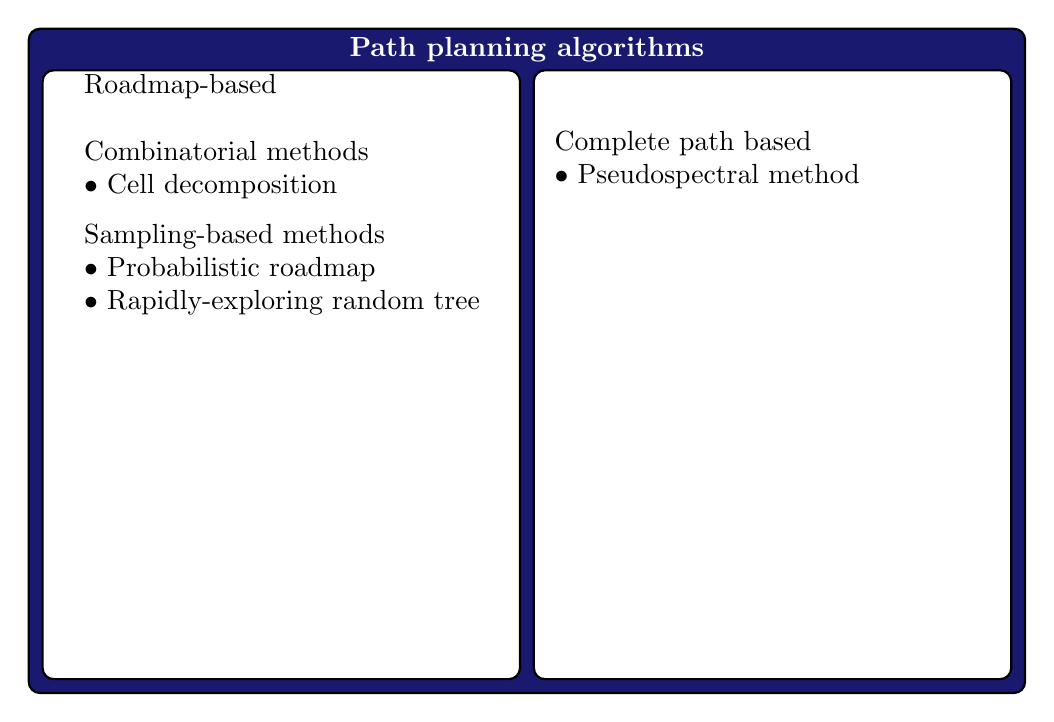
\begin{tikzpicture}[x=1em,y=1em]

	\tikzstyle{block} = [rectangle, draw, thick, fill=white,
    		text centered, rounded corners]
	\tikzstyle{block_marked} = [block, fill=MidnightBlue, text=white, font=\bfseries]
	\tikzstyle{text_marked} = [text=white, font=\bfseries]

    \node [block_marked, minimum height=24em, minimum width=36em] (main) {};
    \node [block, minimum height=22em, minimum width=17.25em] at (-8.875,-0.5) {};
    \node [block, minimum height=22em, minimum width=17.25em] at (8.875,-0.5) {};
    
    \node[text_marked] at (0,11.25) {Path planning algorithms};
   % \node[text width=10em] at (-8,0) {Roadmap-based };
	 \node[text width=15em] at (-8.5,6) {
    		Roadmap-based \\
    		 \bigskip
    		Combinatorial methods \\
  		$\bullet$ Cell decomposition \\
  		\medskip
  		Sampling-based methods \\
  		$\bullet$ Probabilistic roadmap \\
  		$\bullet$ Rapidly-exploring random tree \\
  		
	};
	\node[text width=15em] at (8.5,7.25) {
    		Complete path based \\
  		$\bullet$ Pseudospectral method
	};
   
\end{tikzpicture}